
\documentclass[oneside,a4paper,12pt]{book}

 %%%%%%%%%%%%  Include Packages  %%%%%%%%%%%%%%


\usepackage{fancyhdr}
\fancypagestyle{plain}{%
 \fancyhf{}
 \fancyfoot[CE]{Pune Institute of Computer Technology, Department of Computer Engineering 2021-22}
 \fancyfoot[RE]{\thepage}
}
\pagestyle{fancy}
\fancyhead{}
\renewcommand{\headrulewidth}{0pt}
\footskip = 0.625in
\cfoot{}
\rfoot{}
\usepackage{titlesec}
\usepackage[nottoc,notlot,notlof,numbib]{tocbibind}
\usepackage[titletoc]{appendix}
\usepackage{titletoc}
\renewcommand{\appendixname}{Annexure}
\renewcommand{\bibname}{References}
\usepackage{txfonts}
\usepackage[]{geometry}
\setlength\arrayrulewidth{0pt}
% Blank space below is for aesthetics purpose only
\usepackage{amsmath}
\usepackage{latexsym}
\usepackage{amsfonts}
\usepackage[normalem]{ulem}
\usepackage{array}
\usepackage{amssymb}
\usepackage{graphicx}
\usepackage[backend=biber,
style=numeric,
sorting=none,
isbn=false,
doi=false,
url=false,
]{biblatex}\addbibresource{bibliography.bib}

\usepackage{subfig}
\usepackage{wrapfig}
\usepackage{wasysym}
\usepackage{enumitem}
\usepackage{adjustbox}
\usepackage{ragged2e}
\usepackage[svgnames,table]{xcolor}
\usepackage{tikz}
\usepackage{longtable}
\usepackage{changepage}
\usepackage{setspace}
\usepackage{hhline}
\usepackage{multicol}
\usepackage{tabto}
\usepackage{float}
\usepackage{multirow}
\usepackage{makecell}
\usepackage[hidelinks]{hyperref}
\usetikzlibrary{shapes.symbols,shapes.geometric,shadows,arrows.meta}
\tikzset{>={Latex[width=1.5mm,length=2mm]}}
\usepackage{flowchart}\usepackage[utf8]{inputenc}
\usepackage[T1]{fontenc}
\TabPositions{0.5in,1.0in,1.5in,2.0in,2.5in,3.0in,3.5in,4.0in,4.5in,5.0in,5.5in,6.0in,}

\urlstyle{same}


 %%%%%%%%%%%%  Set Depths for Sections  %%%%%%%%%%%%%%

% 1) Section
% 1.1) SubSection
% 1.1.1) SubSubSection
% 1.1.1.1) Paragraph
% 1.1.1.1.1) Subparagraph


\setcounter{tocdepth}{5}
\setcounter{secnumdepth}{5}


 %%%%%%%%%%%%  Set Depths for Nested Lists created by \begin{enumerate}  %%%%%%%%%%%%%%


\setlistdepth{9}
\renewlist{enumerate}{enumerate}{9}
		\setlist[enumerate,1]{label=\arabic*)}
		\setlist[enumerate,2]{label=\alph*)}
		\setlist[enumerate,3]{label=(\roman*)}
		\setlist[enumerate,4]{label=(\arabic*)}
		\setlist[enumerate,5]{label=(\Alph*)}
		\setlist[enumerate,6]{label=(\Roman*)}
		\setlist[enumerate,7]{label=\arabic*}
		\setlist[enumerate,8]{label=\alph*}
		\setlist[enumerate,9]{label=\roman*}

\renewlist{itemize}{itemize}{9}
		\setlist[itemize]{label=$\cdot$}
		\setlist[itemize,1]{label=\textbullet}
		\setlist[itemize,2]{label=$\circ$}
		\setlist[itemize,3]{label=$\ast$}
		\setlist[itemize,4]{label=$\dagger$}
		\setlist[itemize,5]{label=$\triangleright$}
		\setlist[itemize,6]{label=$\bigstar$}
		\setlist[itemize,7]{label=$\blacklozenge$}
		\setlist[itemize,8]{label=$\prime$}

\setlength{\topsep}{0pt}\setlength{\parskip}{9.96pt}
\setlength{\parindent}{0pt}

 %%%%%%%%%%%%  This sets linespacing (verticle gap between Lines) Default=1 %%%%%%%%%%%%%%


\renewcommand{\arraystretch}{1.3}


%%%%%%%%%%%%%%%%%%%% Document code starts here %%%%%%%%%%%%%%%%%%%%



\begin{document}

\vspace{\baselineskip}
\begin{Center}
\textbf{A PRELIMINARY REPORT ON}
\end{Center}\par

\begin{Center}
{\fontsize{16pt}{19.2pt}\selectfont \textbf{{Medical Image Analysis: Brain tumor Detection and Segmentation.}\par}
\end{Center}\par


\vspace{\baselineskip}
\setlength{\parskip}{0.0pt}
\begin{Center}
SUBMITTED TO THE SAVITRIBAI PHULE PUNE UNIVERSITY, PUNE
\end{Center}\par

\begin{Center}
IN THE PARTIAL FULFILLMENT OF THE REQUIREMENTS
\end{Center}\par

\begin{Center}
FOR THE AWARD OF THE DEGREE
\end{Center}\par

\begin{Center}
OF
\end{Center}\par



\setlength{\parskip}{9.96pt}
\begin{Center}
{\fontsize{16pt}{19.2pt}\selectfont \textbf{BACHELOR OF ENGINEERING (COMPUTER ENGINEERING)}\par}
\end{Center}\par

\begin{Center}
{\fontsize{14pt}{16.8pt}\selectfont \textbf{BY}\par}
\end{Center}\par



%%%%%%%%%%%%%%%%%%%% Table No: 1 starts here %%%%%%%%%%%%%%%%%%%%


\begin{table}[H]
 			\centering
\begin{tabular}{p{3.01in}p{3.01in}}
%row no:1
\multicolumn{1}{p{3.01in}}{\Centering \textbf{JAYESH BHALCHIM} \par \Centering \textbf{SANKET BHATLAWANDE } \par \Centering \textbf{AMISHA GOKHALE}\par \centering
\textbf{VARUN PATIL}} & 
\multicolumn{1}{p{3.01in}}{\Centering Seat No.\textbf{ 41435} \par \Centering Seat No.\textbf{ 41415} \par \Centering Seat
No.\textbf{ 41428} \par \Centering Seat
No.\textbf{ 41459}} \\
\hhline{~~}
%row no:2
\multicolumn{1}{p{3.01in}}{} & 
\multicolumn{1}{p{3.01in}}{} \\
\hhline{~~}

\end{tabular}
 \end{table}
\vspace{\baselineskip}


%%%%%%%%%%%%%%%%%%%% Table No: 1 ends here %%%%%%%%%%%%%%%%%%%%
\vspace{-1.5cm}



%%%%%%%%%%%%%%%%%%%% Figure/Image No: 1 starts here %%%%%%%%%%%%%%%%%%%%

\begin{figure}[H]
	\begin{Center}
		
\includegraphics[width=1.0 in,height=1.0in]{./pict.eps}
	\end{Center}
\end{figure}


%%%%%%%%%%%%%%%%%%%% Figure/Image No: 1 Ends here %%%%%%%%%%%%%%%%%%%%

\par

\setlength{\parskip}{0.0pt}
\begin{Center}
{\fontsize{16pt}{19.2pt}\selectfont \textbf{DEPARTMENT OF COMPUTER ENGINEERING}\par}
\end{Center}\par


\vspace{\baselineskip}

\begin{Center}
{\fontsize{14pt}{16.8pt}\selectfont \textbf{PUNE INSTITUTE OF COMPUTER TECHNOLOGY}\par}
\end{Center}\par


\vspace{\baselineskip}

\begin{Center}
{\fontsize{14pt}{16.8pt}\selectfont \textbf{DHANKAWADI, PUNE-411043}\par}
\end{Center}\par

\vspace{\baselineskip}
% \setlength{\parskip}{0.0pt}
% \setlength{\parskip}{9.96pt}
\begin{Center}
{\fontsize{14pt}{16.8pt}\selectfont \textbf{SAVITRIBAI PHULE PUNE UNIVERSITY}\par}
\end{Center}\par

\begin{Center}
{\fontsize{14pt}{16.8pt}\selectfont\textbf{2021-22}\par}
\end{Center}\par

\( \newpage \)\par

%%%%%%%%%%%%%%%%%%%% Figure/Image No: 2 starts here %%%%%%%%%%%%%%%%%%%%

\begin{figure}[H]
	\begin{Center}
		
\includegraphics[width=1.11in,height=1.11in]{./pict.eps}
	\end{Center}
\end{figure}


%%%%%%%%%%%%%%%%%%%% Figure/Image No: 2 Ends here %%%%%%%%%%%%%%%%%%%%

\par

\begin{Center}
{\fontsize{16pt}{19.2pt}\selectfont \textbf{ CERTIFICATE}\par}
\end{Center}\par


% \vspace*{-1cm}

\vspace{\baselineskip}
\begin{Center}
This is to certify that the Project report entitled
\end{Center}\par

\begin{Center}
\textbf{Medical Image Analysis: Brain tumor Detection and Segmentation}
\end{Center}\par

\begin{Center}
Submitted by
\end{Center}\par



%%%%%%%%%%%%%%%%%%%% Table No: 2 starts here %%%%%%%%%%%%%%%%%%%%


\begin{table}[H]
 			\centering
\begin{tabular}{p{3.01in}p{3.01in}}
%row no:1
\multicolumn{1}{p{3.01in}}{\Centering AMISHA GOKHALE \par \Centering SANKET BHATLAWANDE \par \Centering JAYESH BHALCHIM \par \Centering VARUN PATIL} & 
\multicolumn{1}{p{3.01in}}{\Centering Seat No.\textbf{ }41428 \par \Centering Seat No.\textbf{ }41415 \par \Centering Seat
No.\textbf{ }41435 \par \Centering Seat
No.\textbf{ }41459} \\
\hhline{~~}

\end{tabular}
 \end{table}


%%%%%%%%%%%%%%%%%%%% Table No: 2 ends here %%%%%%%%%%%%%%%%%%%%


\vspace{\baselineskip}

\vspace*{-1cm}
\begin{justify}
are\  bonafide students of this institute and the work has been carried out by them under the supervision of  \textbf{Prof. Dipali Kadam} and it is approved for the partial fulfillment of the requirement of Savitribai Phule Pune University, for the award of the degree of \textbf{Bachelor of Engineering} (Computer Engineering).
\end{justify}\par
\vspace{\baselineskip}




%%%%%%%%%%%%%%%%%%%% Table No: 3 starts here %%%%%%%%%%%%%%%%%%%%


\begin{table}[H]
 			\centering
\begin{tabular}{p{3.01in}p{3.01in}}
%row no:1
\multicolumn{1}{p{3.01in}}{\Centering \textbf{(Prof.Kopal Gangarde)}} & 
\multicolumn{1}{p{3.01in}}{\Centering \textbf{(Dr. Geetanjali Kale)}} \\
\hhline{~~}
%row no:2
\multicolumn{1}{p{3.01in}}{\Centering Internal Guide} & 
\multicolumn{1}{p{3.01in}}{\Centering Head} \\
\hhline{~~}
%row no:3
\multicolumn{1}{p{3.01in}}{\Centering Department. of Computer Engineering} & 
\multicolumn{1}{p{3.01in}}{\Centering Department. of Computer Engineering} \\
\hhline{~~}

\end{tabular}
 \end{table}
\vspace{\baselineskip}


%%%%%%%%%%%%%%%%%%%% Table No: 3 ends here %%%%%%%%%%%%%%%%%%%%

\setlength{\parskip}{0.0pt}
\begin{Center}
\textbf{(Dr. R. Sreemathy)}
\end{Center}\par

\begin{Center}
Principal
\end{Center}\par

\begin{Center}
Pune Institute of Computer Technology
\end{Center}\par



%%%%%%%%%%%%%%%%%%%% Table No: 4 starts here %%%%%%%%%%%%%%%%%%%%



%%%%%%%%%%%%%%%%%%%% Table No: 4 ends here %%%%%%%%%%%%%%%%%%%%


\vspace{\baselineskip}
\setlength{\parskip}{9.96pt}
Place: Pune\par

Date: \par


\frontmatter
\cfoot{P.I.C.T., Department of Computer Engineering 2021-22\newline\thepage}
\setlength\arrayrulewidth{0.5pt}
\pagenumbering{Roman}
\begin{adjustwidth}{1.5in}{0.0in}
{\fontsize{14pt}{16.8pt}\selectfont \textbf{ACKNOWLEDGEMENT}\par}\par

\end{adjustwidth}


\vspace{\baselineskip}
It gives us great pleasure in presenting the preliminary project report on \textbf{\textit{Medical Image Analysis: Brain tumor Detection and Segmentation}}\par

We would like to take this opportunity to thank our internal guide \textbf{Proj. Kopal Gangarde} for giving us all the help and guidance we needed. We are really grateful to him for his kind support. Her valuable suggestions were very helpful.\par

We are also grateful to \textbf{\textit{Dr. Geetanjali Kale}}\textit{,} Head of \textbf{ Department of Computer Engineering,}
\textbf{Pune Institute of Computer Technology} for his indispensable support and suggestions.\par


\vspace{\baselineskip}

\vspace{\baselineskip}


%%%%%%%%%%%%%%%%%%%% Table No: 5 starts here %%%%%%%%%%%%%%%%%%%%


\begin{table}[H]
 			\centering
\begin{tabular}{p{3.01in}p{3.01in}}
%row no:1
\multicolumn{1}{p{3.01in}}{} & 
\multicolumn{1}{p{3.01in}}{\Centering AMISHA GOKHALE} \\
\hhline{~~}
%row no:2
\multicolumn{1}{p{3.01in}}{} & 
\multicolumn{1}{p{3.01in}}{\Centering SANKET BHATLAWANDE} \\
\hhline{~~}
%row no:3
\multicolumn{1}{p{3.01in}}{} & 
\multicolumn{1}{p{3.01in}}{\Centering JAYESH BHALCHIM} \\
%row no:4
\multicolumn{1}{p{3.01in}}{} & 
\multicolumn{1}{p{3.01in}}{\Centering VARUN PATIL} \\
\hhline{~~}

%row no:5
\multicolumn{1}{p{3.01in}}{} & 
\multicolumn{1}{p{3.01in}}{\Centering (B.E. Computer Engg.)} \\
\hhline{~~}

\end{tabular}
 \end{table}


%%%%%%%%%%%%%%%%%%%% Table No: 5 ends here %%%%%%%%%%%%%%%%%%%%


\vspace{\baselineskip}

\vspace{\baselineskip}

\vspace{\baselineskip}
\( \newpage \)\par


\vspace{\baselineskip}

\vspace{\baselineskip}
\begin{Center}
{\fontsize{14pt}{16.8pt}\selectfont \textbf{ABSTRACT}\par}
\end{Center}\par

 \( \hspace{0.5cm}\) 
 Medical diagnosis/detection of diseases with the help of image processing, computer vision and machine learning are considered one of the most prominent issues
in artificial intelligence. Similarly, Deep learning, which is considered as part of
machine learning has gained importance in almost every field where “decision making” is comprised especially in the field of health care. The concept of artificial
intelligence has shown encouraging results in disease/virus diagnosis with image
processing.
\par
\( \hspace{0.5cm}\)In recent year, the brain imaging techniques has regularly vie a necessary role in inspecting and concentrating on new visions of anatomy and brain functions. The image process mechanism is extensively employed in drugs to reinforce early detection and treatment. Segmentation and classification is significant role for imaging brain image processing. The aim of this work is to develop a system that helps in tumor detection and brain MRI image recognition through the method of the planned image classifier. during this work, we have a tendency to advocate a Deep Neural Network for classification and segmentation. This work proposes a picture compression technique mistreatment a Deep rippling machine encoder (DWA) that mixes the flexibility to attenuate the first perform of automatic encoders with the image degradation property of the wavelet transform. the mixture of the 2 has a necessary impact on reducing the scale of the function set to face up to additionally classification tasks with DNN. A brain system has been eliminated and therefore the planned DNN- DWAE image classification is considered. The performance analysis for the DNN- DWAE classifier has been improved compared with totally different existing method.

Keywords: Deep neural network, Denoising autoencoder, segmentation, tumour detection.



 %%%%%%%%%%%%  Starting New Page here %%%%%%%%%%%%%%

\newpage

\vspace{\baselineskip}
\vspace{\baselineskip}

% Following code generates Table Of Contents
% List Of Figures
% and Table Of Tables
\tableofcontents
\listoffigures




\mainmatter


% Following code will place chapter titles in the center of the
% page
\titleformat{\chapter}[display]
{\fontsize{16}{15}\filcenter}
{\vspace*{\fill}
\bfseries\LARGE\MakeUppercase{\chaptertitlename}~\thechapter}
{1pc}
{\bfseries\LARGE\MakeUppercase}
[\thispagestyle{empty}\vspace*{\fill}\newpage]






















\vspace{\baselineskip}

\vspace{\baselineskip}

\vspace{\baselineskip}
\chapter{INTRODUCTION}\par


\vspace{\baselineskip}


 %%%%%%%%%%%%  Starting New Page here %%%%%%%%%%%%%%

\newpage

\vspace{\baselineskip}\section*{1.1\hspace*{10pt}Motivation}
\addcontentsline{toc}{section}{1.1\hspace*{10pt}Motivation}
    \( \hspace{0.5cm}\)The motivation behind the detection of brain tumor also extends to the classification of the same. This early detection of the tumor can result a better recovery for the patient and a better analysis system for the doctor.
The percentage of confidence of the model in a particular result will also state if further inspection is needed on the case. Apart from the detection, these details will make a patients case easier for the doctor to take a look at. This saves time and money both for both the sides.
\par
    \( \hspace{0.5cm}\)Having brain tumours is a critical condition and can be fatal if not detected early and treated. Increase in fatality rates because of CNS tumor is an
alarm for an efficient segmentation. This has become a crucial task in medical image analysis and is often the first and most crucial step in a good deal of clinical
diagnosis.
\par

\section*{1.2\hspace*{10pt}Problem Definition}
\addcontentsline{toc}{section}{1.2\hspace*{10pt}Problem Definition}
 \( \hspace{0.5cm}\)\
 In existing non deep learning methodology ,the main downside of growth detection of images are,Poor discriminatory power, High process load, Loss of edge details because of shift variant property and fewer accuracy in classification Medical Resonance images contain a noise caused by operator performance which might result in serious inaccuracies classification.
\par


\vspace{\baselineskip}

\vspace{\baselineskip}

\vspace{\baselineskip}

\vspace{\baselineskip}

\vspace{\baselineskip}

\vspace{\baselineskip}

\vspace{\baselineskip}

\vspace{\baselineskip}

\vspace{\baselineskip}

\vspace{\baselineskip}
\chapter{LITERATURE SURVEY}\par


 %%%%%%%%%%%%  Starting New Page here %%%%%%%%%%%%%%

\newpage
\vspace{\baselineskip}\section*{2.1\hspace*{10pt} Wavelet autoencoder based brain tumor detection analysis using DNN
}
\addcontentsline{toc}{section}{2.1\hspaceGlobal  A Wavelet autoencoder based brain tumor detection analysis using DNN}
\begin{enumerate}

\item Author :T.Balamurugan, E.Gnanamanoharan, L.Martin     

\item Aim : The aim of this work is to develop a system that helps in tumour detection and brain MRI image recognition through the process of the proposed image classifier. 
\item Result : Ultrasonic and MRI images were used for achieving better image enhancing and preserving the image textures.
In this work, Deep Neural Network is used for classification and segmentation. This work proposes an image compression technique using a Deep Wavelet Auto encoder (DWA) that combines the ability to minimize the primary function of automatic encoders with the image degradation property of the wavelet transform.


\item Conclusion : In this work, an unsupervised exploratory was used where efficient de-noising enhancing edge detection and preserving details.
The combination of the two has an essential impact on reducing the size of the function set to withstand in addition classification tasks with DNN. A brain system has been eliminated and the proposed DNN- DWAE image classification is considered.


\end{enumerate}\par

\newpage

\vspace{\baselineskip}\section*{2.2\hspace*{10pt}: 3-D MRI brain tumor segmentation using Auto Encoder regularization.  }
\addcontentsline{toc}{section}{2.2\hspace*{10pt}3-D MRI brain tumor segmentation using Auto Encoder regularization. }
\begin{enumerate}
\item Author : Andriy Myronenko

\item Aim : To procure high intensity CT lung image
\item Result : They described a semantic segmentation network for brain tumor segmentation from multimodal 3D MRIs. 
\item Conclusion : In this study,n this paper, we have investigated the different Entropy functions for tumor segmentation and its detection from various MRI images. The different threshold values are obtained depend on the particular definition of the entropy. The threshold values are dependent on the different entropy function which in turn affects the segmented results.
Using the NVIDIA 32GB GPU they were able to double the number of features compared to 16GB version. Finally, the additional VAE branch helped to regularize the shared encoder, which not only improved the performance, but helped to consistently achieve good training accuracy.

\end{enumerate}
\par
\newpage
\vspace{\baselineskip}\section*{2.3\hspace*{10pt}An efficient Brain Tumor Detection from MRI Images using Entropy Measures }
\addcontentsline{toc}{section}{2.3\hspace*{10pt}An efficient Brain Tumor Detection from MRI Images using Entropy Measures }
\begin{enumerate}

\item Author : Devendra Somwanshi , Ashutosh Kumar, Pratima Sharma, Deepika Joshi

\item Aim :Detecting tumor using entropy measures
\item Result :Here, ultrasonic images,MRI,CT,X-ray are being targetted to imrpove texture and smooth the forbidden area of the images.The contrast of the medical images improved for better medical imaging diagnosis.\par Here they have have investigated the different Entropy functions for tumor segmentation and its detection from various MRI images. The different threshold values are obtained depend on the particular definition of the entropy. The threshold values are dependent on the different entropy function which in turn affects the segmented results.

\item Conclusion :  
Here they have have investigated the different Entropy functions for tumor segmentation and its detection from various MRI images. The different threshold values are obtained depend on the particular definition of the entropy. The threshold values are dependent on the different entropy function which in turn affects the segmented results.
\end{enumerate}

\newpage
\vspace{\baselineskip}\section*{2.4\hspace*{10pt}A Review on Brain Tumor Detection and Segmentation: Inferences, Key Achievements and Future Road Map }
\addcontentsline{toc}{section}{2.4\hspace*{10pt}A Review on Brain Tumor Detection and Segmentation: Inferences, Key Achievements and Future Road Map}
\begin{enumerate}

\item Author :Devendra Somwanshi , Ashutosh Kumar, Pratima Sharma, Deepika Joshi
\item Aim : The model that we propose is a combination of Deep
learning and Image Processing techniques for detection
and segmentation of tumor.
\item Result :This system will be capable of performing
everything right from tumor detection, segmentation,
area calculation, and also classification of the tumor
thereby reducing the human error to a large extent and
will help in on-time detection of the tumor.Though the
computation time increases, our proposed model will
give accurate results.
\item Conclusion :  
Combination of all these methods in collaboration with
Transfer learning will help in building a highly
automated, accurate, robust system for tumor
detection.
In the future scope, survival
prediction of the patient can also be made possible.
\end{enumerate}

\newpage
\vspace{\baselineskip}\section*{2.5\hspace*{10pt}Edge based active contour method}
\addcontentsline{toc}{section}{2.5\hspace*{10pt}Edge based active contour method}
\begin{enumerate}

\item Author :Deep Gupta
\item Aim :Edge based active contour method and clustering technique.
\item Result :This paper surveys the various techniques that are part of Medical Image Processing and are prominently used in discovering brain tumors from MRI Images. It has used MRI of skull and brain to detect a disease called as tuberculoma and also to detect some prostatic carcinoma on which segmentation would be performed.
\item Conclusion :  
: Pros: It Accurately shows the results and also it eliminates the manual requriement and also decreases the processing time needed for execution.
Cons: Algorithm complexity is more, also some relevant images missed as they used the diverse density relevance feedback algorithm. Also manual intervention is required.
\end{enumerate}
\newpage
\vspace{\baselineskip}\section*{2.6\hspace*{10pt}A dual Autoencoder and singular value decomposition based feature optimization for  segmentation of brain tumor from MRI images.
}
\addcontentsline{toc}{section}{2.6\hspace*{10pt}A dual Autoencoder and singular value decomposition based feature optimization for  segmentation of brain tumor from MRI images.
}
\begin{enumerate}

\item Author :K. Aswani And D.Menaka

\item Aim : Combining MRI and CT diagnosing for tumor.
\item Result : The results present here are obtained by using the patch size of MRI images of dimensions 16 x 64 x 16 for horizontal and vertical patches. In the images pre-processed Glioma Tumor is not something grown from a particular point but rather spreads, so here region filling and connectivty operations/morphological operations are being carried out here to get the final tumor segmentation to measure the performance on the metrics such as Dice Similarity Coefficient, positive predictive value and the sensitivity.
\item Conclusion :  
Here an unsupervised method for the segmentation of brain tumor was being used which were collected from the brain MRI images . The proposed dual AE is useful for the process of dimensionality reduction due to which, no huge database is required for one to have a better accuracy unlike SVM , KNN machine learning methods.
\end{enumerate}

\setlength{\parskip}{9.96pt}

\vspace{\baselineskip}

\vspace{\baselineskip}

\vspace{\baselineskip}

\vspace{\baselineskip}

\vspace{\baselineskip}

\vspace{\baselineskip}

\vspace{\baselineskip}

\vspace{\baselineskip}

\vspace{\baselineskip}

\vspace{\baselineskip}

\vspace{\baselineskip}

\vspace{\baselineskip}

\vspace{\baselineskip}

\vspace{\baselineskip}

\vspace{\baselineskip}
\chapter{SOFTWARE REQUIREMENTS SPECIFICATION}\par



 %%%%%%%%%%%%  Starting New Page here %%%%%%%%%%%%%%

\newpage

\vspace{\baselineskip}\section*{3.1\hspace*{10pt}Introduction}
\addcontentsline{toc}{section}{3.1\hspace*{10pt}Introduction}
\par
Whenever a person is diagnosed with a disease or any kind of unknown health-related problems. A patient always seeks a third party advice from his/her friends or relatives because he/she is unaware of which hospital or doctor to refer for the best treatment. Often this kind of suggestions are not reliable and may lead to time delay which is very crucial in times of emergency. If we have a recommendation system in place, this type of situations can be avoided thus providing appropriate medication at right time. 
\par
Now even though the user knows which hospital/doctor to visit, he/she may have to carry all the previous medical history documents with them which is not absolutely feasible at all times. This data can be recorded on a platform and can be used for future purpose whenever required. 
\subsection*{3.1.1\hspace*{10pt}Project Scope}
\addcontentsline{toc}{subsection}{3.1.1\hspace*{10pt}Project Scope}



 1)\textbf{Detection:} of brain tumor with the input of Head MRI images by using Deep Learning. Further extending this use case by attempting to modify/optimize the chosen model, so as to create an optimal model for Head MRIs.\par 2) \textbf{Classification:} Our final result will consist of a website/webapp that helps to predict the results after uploading the MRIs.
\par

\par





\subsection*{3.1.2\hspace*{10pt}Assumptions and Dependencies}
\addcontentsline{toc}{subsection}{3.1.3\hspace*{10pt}Assumptions and Dependencies}
\( \hspace{0.5cm}\)\ \textbf{Assumptions} :
\begin{enumerate}
	\item 	We assume that we have optimal data that can be trained, after basic cleaning and preprocessing.\par

	\item 	Sufficient resources are available for the final training and optimization of the model. \par
	
	\item 	We have sufficient amount of data that will be enough to train the model optimally.\par
	
\end{enumerate}\par
\newpage
\textbf{Dependencies :}
\begin{enumerate}
    \item 	We have only considered the case of detecting brain tumors only with Head MRI inputs, other factors in detection are not considered.
    
    
    
    .
\end{enumerate}\par
\subsection*{3.1.3\hspace*{10pt}Constraints}

\begin{enumerate}
	\item 	The classes that can be detected and classified are postcontrast T1-weighted MRI scans by tumor classes (high-grade glioma, low-grade glioma [LGG], brain metastasis, meningioma, pituitary adenoma, and acoustic neuroma) and a healthy tissue (HLTH) class.
	\end{enumerate}\par
\section*{3.2\hspace*{10pt}Functional requirements}
\addcontentsline{toc}{section}{3.2\hspace*{10pt}Functional requirements}
\subsection*{3.2.1\hspace*{10pt}Input Dataset}
 \item
We need to preprocess the data and prepare it for training using techniques like rescaling; data augmentation aimed either to improve image quality or to standardize its geometric and intensity patterns.

\par
\item
The datasets used for the analysis are post contrast T1-weighted MR scans from four publicly available datasets; the Brain Tumor Image Segmentation dataset, Cancer Genome Atlas Glioblastoma Multiform dataset, and The Cancer Genome Atlas Low Grade Glioma dataset and the LGG-1p19q dataset.
\par


\vspace{\baselineskip}
\subsection*{3.2.2\hspace*{10pt}Transformed results after training}
\item
	   \hspace{0.5}1) The final results should be such that they provide a good solution to the problem statement after filtering and segmentation of the data. The solution should help in detecting an early brain tumor. 
	The result when we give an image to the program is a probability that the brain contains a tumor, so we could prioritize the patients who have a higher probability of a positive result.



\section*{3.3\hspace*{10pt}Non-Functional requirements}
\addcontentsline{toc}{section}{3.3\hspace*{10pt}Non-Functional requirements}
\subsection*{3.3.1\hspace*{10pt}Performance Requirement}
\addcontentsline{toc}{subsection}{3.3.1\hspace*{10pt}Performance Requirement}
\begin{enumerate}
    	\item User satisfaction:\par	 The system should be able to determine the confidence of the predicted result so the doctor can analyze it further if needed. 
    	\item 	Response time: \parAfter the training, the model should be able to update itself and predict the input data faster than it takes to physically analyze the report today.
    	\item Application availability:\par The application should be up and running with minimum downtime


	\
\end{enumerate}\par



\subsection*{3.3.2\hspace*{10pt}Software Quality Attributes}
\addcontentsline{toc}{subsection}{3.3.4\hspace*{10pt}Software Quality Attributes}
\begin{enumerate}
	\item \textcolor[HTML]{222222}{Accuracy:}\par There should be at least a delta improvement in the performance of the model after addition of more training data, that will get updated as users use the system, and the model will be trained more.


	\item \textcolor[HTML]{222222}{Reliability:}\par It is desired that the predictions of the systems are reliable with a high accuracy and precision. 

	\item \textcolor[HTML]{222222}{ Learnability:}\par The learnability of a software system is determined by the user interface design as well as the clarity and simplicity of the user instructions (tutorial or user manual).
	
	\item \textcolor[HTML]{222222}{ Speed:}\par System deployment should be such that results are delivered in minimal time





	
\end{enumerate}\par

\vspace{\baselineskip}
\section*{3.4\hspace*{10pt}External Interface Requirements}
\addcontentsline{toc}{section}{3.4\hspace*{10pt}External requirements}
\subsection*{3.4.1\hspace*{10pt}User Interface}
\addcontentsline{toc}{subsection}{3.4.1\hspace*{10pt}User Interface}
\item
1.) Web or software application for doctors/electronic health record handlers, that can predict the results after uploading an MRI image
\item
2.) In the future, the deployment can be extended to mobile applications aswell. UI for central server administrator to look into the updates in training model.
\vspace{\baselineskip}
\section*{3.5\hspace*{10pt}System Requirements}
\addcontentsline{toc}{section}{3.4\hspace*{10pt}System Requirements}
\subsection*{3.5.1\hspace*{10pt}Database Requirements}
\addcontentsline{toc}{subsection}{3.4.1\hspace*{10pt}Database Requirements}
 1.)	The data can be initially stored on the cloud. Later, the data should be stored on the server for updating purposes.\par
\newpage
\subsection*{3.5.2\hspace*{10pt}Software Requirements}
\addcontentsline{toc}{subsection}{3.4.2\hspace*{10pt}Software Requirements}
\begin{enumerate}
	\item NodeJs / Flask / Django: For implementing the backend of the web application. Flask is used for writing web services. 

	\item PyTorch: PyTorch is a deep learning framework written in Python useful for building deep learning architectures. \par
	
	\item Keras: Python API used as an interface for artificial neural networks
	
	\item Scikit-learn / Pandas / Numpy: Supporting libraries in Python useful for data analysis and preprocessing.

\end{enumerate}\par

\subsection*{3.5.3\hspace*{10pt}Hardware Requirements}
\addcontentsline{toc}{subsection}{3.4.3\hspace*{10pt}Hardware Requirements}
\begin{enumerate}
	\item Processor (i5 or higher): Fast and efficient systems are needed to handle intensive loads and provide efficient throughput.\par

	\item RAM (8GB minimum): Helps in performing fast computations and optimizes execution process.\par
	
	\item Hard disk: 10 GB of available space or more.
\item Operating system: Windows

	
\end{enumerate}\par





\begin{Center}


%%%%%%%%%%%%%%%%%%%% Figure/Image No: 4 starts here %%%%%%%%%%%%%%%%%%%%







%%%%%%%%%%%%%%%%%%%% Figure/Image No: 4 Ends here %%%%%%%%%%%%%%%%%%%%

\\

\end{Center}\par
\newpage
\section*{3.6\hspace*{10pt}Algorithm}
\item Step1: Pre-processing of DICOM images to extract the specific image matrix only. 
\item Step2: Flattening of image matrices to construct image dataset. 
\item Step3: Splitting of dataset to sub arrays 
\item Step4: for each sub array continue the steps 5 to 9 
\item Step5: Input the image sub array to Deep Wavelet Autoencoder for encoding 
\item Step6: Pass the encoded image through low pass and high pass filter using discrete wavelet transform for decomposition. 
\item Step7: Apply inverse wavelet transform to combine and decode the images to get original image 
\item Step8: Run the Autoencoder for number of epochs to get optimized weight and bias values 
\item Step9: Extract approximation coefficients from the hidden layer, combine them and provide as input to a deep neural network for classification. 
\item Step10: Train the DNN with the inputs provided by step9 and tests the network for different metrics measurement. 
\item Step11: Apply the Train DNN to the Flask Model 
\item Step12: Upload MRI Image to Scan Model to Predict the Different Results.


\addcontentsline{toc}{section}{3.7\hspace*{10pt}Algorithm}

\section*{3.7\hspace*{10pt}System Implementation Plan}
\addcontentsline{toc}{section}{3.7\hspace*{10pt}System Implementation Plan}



\vspace{\baselineskip}

\vspace{\baselineskip}
\setlength{\parskip}{0.0pt}
\setlength{\parskip}{9.96pt}


%%%%%%%%%%%%%%%%%%%% Table No: 7 starts here %%%%%%%%%%%%%%%%%%%%


\begin{table}[H]
 			\centering
\begin{tabular}{p{0.77in}p{3.1in}p{1.65in}}
\hline
%row no:1
\multicolumn{1}{|p{0.77in}}{\textcolor[HTML]{00000A}{SR NO.}} & 
\multicolumn{1}{|p{3.1in}}{\textcolor[HTML]{00000A}{TASK}} & 
\multicolumn{1}{|p{1.65in}|}{\textcolor[HTML]{00000A}{DUE DATE}} \\
\hhline{---}
%row no:2
\multicolumn{1}{|p{0.77in}}{\textcolor[HTML]{00000A}{1.}} & 
\multicolumn{1}{|p{3.1in}}{\textcolor[HTML]{00000A}{Literature survey}} & 
\multicolumn{1}{|p{1.65in}|}{\textcolor[HTML]{00000A}{2nd week of August}} \\
\hhline{---}
%row no:3
\multicolumn{1}{|p{0.77in}}{\textcolor[HTML]{00000A}{2.}} & 
\multicolumn{1}{|p{3.1in}}{\textcolor[HTML]{00000A}{Defining problem statement}} & 
\multicolumn{1}{|p{1.65in}|}{\textcolor[HTML]{00000A}{3rd week of August}} \\
\hhline{---}
%row no:4
\multicolumn{1}{|p{0.77in}}{\textcolor[HTML]{00000A}{3.}} & 
\multicolumn{1}{|p{3.1in}}{\textcolor[HTML]{00000A}{Designing class diagrams, E-R diagrams} \par \textcolor[HTML]{00000A}{and related models}} & 
\multicolumn{1}{|p{1.65in}|}{\textcolor[HTML]{00000A}{3rd week of September}} \\
\hhline{---}
%row no:5
\multicolumn{1}{|p{0.77in}}{\textcolor[HTML]{00000A}{4.}} & 
\multicolumn{1}{|p{3.1in}}{\textcolor[HTML]{00000A}{Review of design}} & 
\multicolumn{1}{|p{1.65in}|}{\textcolor[HTML]{00000A}{4th week of September}} \\
\hhline{---}
%row no:6
\multicolumn{1}{|p{0.77in}}{\textcolor[HTML]{00000A}{5.}} & 
\multicolumn{1}{|p{3.1in}}{\textcolor[HTML]{00000A}{Finding appropriate dataset}} & 
\multicolumn{1}{|p{1.65in}|}{\textcolor[HTML]{00000A}{1st week of November}} \\
\hhline{---}
%row no:7
\multicolumn{1}{|p{0.77in}}{\textcolor[HTML]{00000A}{6.}} & 
\multicolumn{1}{|p{3.1in}}{\textcolor[HTML]{00000A}{Preparation and cleaning of final structured data.}} & 
\multicolumn{1}{|p{1.65in}|}{\textcolor[HTML]{00000A}{3rd week of November}} \\
\hhline{---}
%row no:8
\multicolumn{1}{|p{0.77in}}{\textcolor[HTML]{00000A}{7.}} & 
\multicolumn{1}{|p{3.1in}}{\textcolor[HTML]{00000A}{Visualizing trends and communicating reports}} & 
\multicolumn{1}{|p{1.65in}|}{\textcolor[HTML]{00000A}{1st week of December}} \\
\hhline{---}

%row no:9
\multicolumn{1}{|p{0.77in}}{\textcolor[HTML]{00000A}{8.}} & 
\multicolumn{1}{|p{3.1in}}{\textcolor[HTML]{00000A}{Selecting the appropriate algorithms}} & 
\multicolumn{1}{|p{1.65in}|}{\textcolor[HTML]{00000A}{3rd week of December}} \\
\hhline{---}
%row no:10
\multicolumn{1}{|p{0.77in}}{\textcolor[HTML]{00000A}{9.}} & 
\multicolumn{1}{|p{3.1in}}{\textcolor[HTML]{00000A}{Complete model testing}} & 
\multicolumn{1}{|p{1.65in}|}{\textcolor[HTML]{00000A}{3rd week of February}} \\
\hhline{---}
%row no:11
\multicolumn{1}{|p{0.77in}}{\textcolor[HTML]{00000A}{10.}} & 
\multicolumn{1}{|p{3.1in}}{\textcolor[HTML]{00000A}{Application development.}} & 
\multicolumn{1}{|p{1.65in}|}{\textcolor[HTML]{00000A}{2nd week of March}} \\
\hhline{---}

%row no:12
\multicolumn{1}{|p{0.77in}}{\textcolor[HTML]{00000A}{11.}} & 
\multicolumn{1}{|p{3.1in}}{\textcolor[HTML]{00000A}{Testing of the application.}} & 
\multicolumn{1}{|p{1.65in}|}{\textcolor[HTML]{00000A}{2nd week of March}} \\
\hhline{---}

\end{tabular}
 \end{table}
\addcontentsline{toc}{section}{3.8\hspace*{10pt}Team Organization}

\section*{3.8\hspace*{10pt}Team Organization}
Updates on development of the software is given to the guide on regular basis. Every month a meet is held with the guide to discuss the next project steps in detail.
\addcontentsline{toc}{section}{3.8\hspace*{10pt}Team Organization}
\item•Sanket Bhatlawande - Model Selection, Training and development 
\item•Jayesh Bhalchim - Model Selection, development and Data Pre-processing
\item•Amisha Gokhale-ML model testing and development & documentation.
\item•Varun Patil: Web application designing and development & documentation


%%%%%%%%%%%%%%%%%%%% Table No: 7 ends here %%%%%%%%%%%%%%%%%%%%


\vspace{\baselineskip}
\setlength{\parskip}{0.0pt}
\setlength{\parskip}{9.96pt}

\vspace{\baselineskip}
\setlength{\parskip}{0.0pt}
\setlength{\parskip}{9.96pt}

\vspace{\baselineskip}
\setlength{\parskip}{0.0pt}
\setlength{\parskip}{9.96pt}

\vspace{\baselineskip}
\setlength{\parskip}{0.0pt}
\setlength{\parskip}{9.96pt}

\vspace{\baselineskip}
\setlength{\parskip}{0.0pt}
\setlength{\parskip}{9.96pt}

\vspace{\baselineskip}
\setlength{\parskip}{0.0pt}
\setlength{\parskip}{9.96pt}

\vspace{\baselineskip}
\setlength{\parskip}{0.0pt}
\setlength{\parskip}{9.96pt}

\vspace{\baselineskip}
\setlength{\parskip}{0.0pt}
\setlength{\parskip}{9.96pt}

\vspace{\baselineskip}
\setlength{\parskip}{0.0pt}
\setlength{\parskip}{9.96pt}

\vspace{\baselineskip}
\setlength{\parskip}{0.0pt}
\setlength{\parskip}{9.96pt}

\vspace{\baselineskip}
\setlength{\parskip}{0.0pt}
\setlength{\parskip}{9.96pt}

\vspace{\baselineskip}
\setlength{\parskip}{0.0pt}
\setlength{\parskip}{9.96pt}

\vspace{\baselineskip}
\setlength{\parskip}{0.0pt}
\setlength{\parskip}{9.96pt}

\vspace{\baselineskip}
\setlength{\parskip}{0.0pt}
\setlength{\parskip}{9.96pt}

\vspace{\baselineskip}
\setlength{\parskip}{0.0pt}
\setlength{\parskip}{9.96pt}

\vspace{\baselineskip}
\setlength{\parskip}{0.0pt}
\setlength{\parskip}{9.96pt}

\vspace{\baselineskip}
\setlength{\parskip}{0.0pt}
\setlength{\parskip}{9.96pt}

\vspace{\baselineskip}
\setlength{\parskip}{0.0pt}
\setlength{\parskip}{9.96pt}

\vspace{\baselineskip}
\setlength{\parskip}{0.0pt}
\setlength{\parskip}{9.96pt}

\vspace{\baselineskip}
\setlength{\parskip}{0.0pt}
\setlength{\parskip}{9.96pt}

\vspace{\baselineskip}
\setlength{\parskip}{0.0pt}
\setlength{\parskip}{9.96pt}

\vspace{\baselineskip}
\setlength{\parskip}{0.0pt}
\setlength{\parskip}{9.96pt}

\vspace{\baselineskip}
\setlength{\parskip}{0.0pt}
\setlength{\parskip}{9.96pt}

\vspace{\baselineskip}
\setlength{\parskip}{0.0pt}
\setlength{\parskip}{9.96pt}

\vspace{\baselineskip}
\setlength{\parskip}{0.0pt}
\setlength{\parskip}{9.96pt}

\vspace{\baselineskip}
\setlength{\parskip}{0.0pt}
\setlength{\parskip}{9.96pt}

\vspace{\baselineskip}
\setlength{\parskip}{0.0pt}
\setlength{\parskip}{9.96pt}

\vspace{\baselineskip}
\setlength{\parskip}{0.0pt}
\setlength{\parskip}{9.96pt}

\vspace{\baselineskip}
\setlength{\parskip}{0.0pt}
\setlength{\parskip}{9.96pt}

\vspace{\baselineskip}
\setlength{\parskip}{0.0pt}
\setlength{\parskip}{9.96pt}

\vspace{\baselineskip}
\setlength{\parskip}{0.0pt}
\setlength{\parskip}{9.96pt}

\vspace{\baselineskip}
\setlength{\parskip}{0.0pt}
\setlength{\parskip}{9.96pt}

\vspace{\baselineskip}
\setlength{\parskip}{0.0pt}
\setlength{\parskip}{9.96pt}

\vspace{\baselineskip}
\setlength{\parskip}{0.0pt}
\setlength{\parskip}{9.96pt}

\vspace{\baselineskip}
\setlength{\parskip}{0.0pt}
\setlength{\parskip}{9.96pt}

\vspace{\baselineskip}
\setlength{\parskip}{0.0pt}
\setlength{\parskip}{9.96pt}

\vspace{\baselineskip}
\setlength{\parskip}{0.0pt}
\setlength{\parskip}{9.96pt}

\vspace{\baselineskip}
\setlength{\parskip}{0.0pt}
\setlength{\parskip}{9.96pt}

\vspace{\baselineskip}

\vspace{\baselineskip}
\chapter{SYSTEM DESIGN}\par



 %%%%%%%%%%%%  Starting New Page here %%%%%%%%%%%%%%

\newpage

\vspace{\baselineskip}\section*{4.1\hspace*{10pt}System Architecture}
\addcontentsline{toc}{section}{4.1\hspace*{10pt}System Architecture}
\vspace{\baselineskip}


\begin{Center}
\begin{figure}[H]
	\begin{Center}
		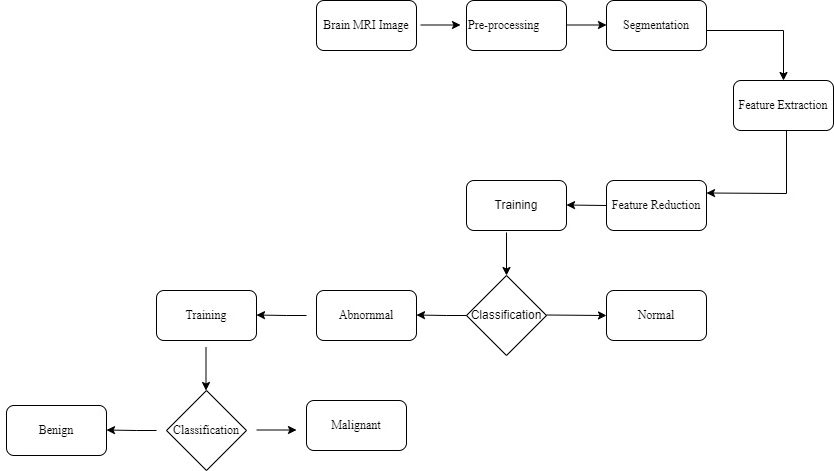
\includegraphics[width=1.1\linewidth]{archi.jpg}
		\caption{Architecture Diagram}
		\label{fig:Architecture_Diagram}
	\end{Center}
\end{figure}
\end{Center}\par



\section*{4.2\hspace*{10pt}Diagram  for Deep-wavelet AE}
\addcontentsline{toc}{section}{4.2\hspace*{10pt} Diagram  for Deep-wavelet Auto-encoder}
\begin{Center}
\begin{figure}[H]
	\begin{Center}
		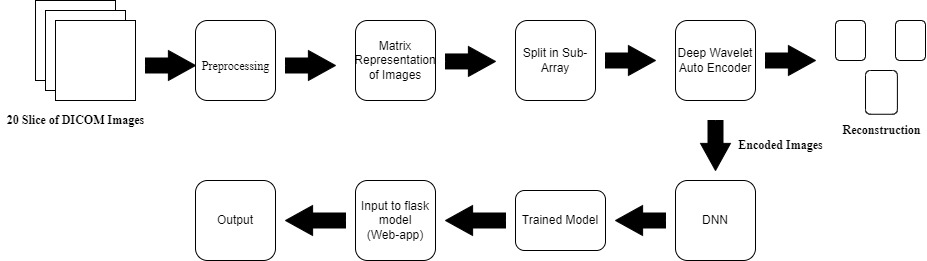
\includegraphics[width=1.0\linewidth]{Deep_wavelet_AE.jpg}
		\caption{DWAE Diagram}
		\label{fig:EndorsersCommitters_Role}
	\end{Center}
\end{figure}
\end{Center}\par


\section*{4.3\hspace*{10pt}Diagram for Denoising  technique}
\addcontentsline{toc}{section}{4.3\hspace*{10pt}Denoising Auto-encoder}
\begin{Center}
\begin{figure}[H]
	\begin{Center}
		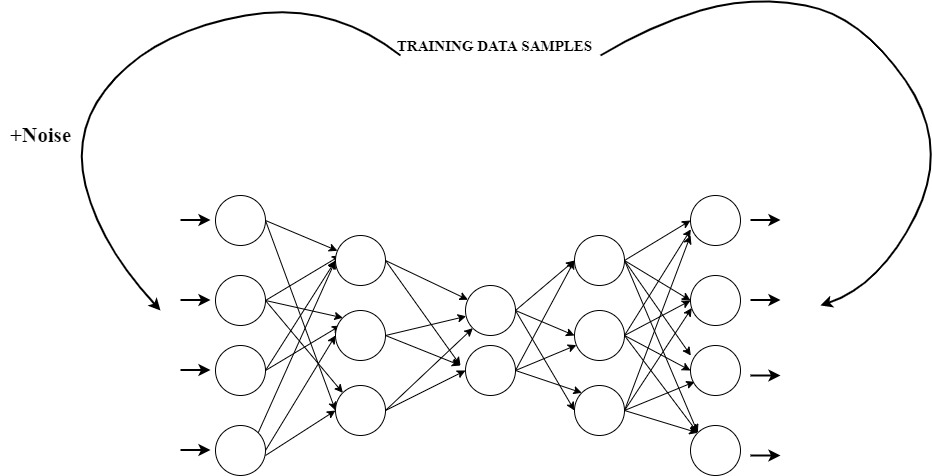
\includegraphics[width=\linewidth]{Denoising_AE.jpg}
		\caption{DFD Diagram}
		\label{fig:EndorsersCommitters_Role}
	\end{Center}
\end{figure}
\end{Center}\par

\section*{4.4\hspace*{10pt} Diagram  for Schematic Auto-Encoder}
\addcontentsline{toc}{section}{4.4\hspace*{10pt} Diagram  for Skull stripping algorithm}
\begin{Center}
\begin{figure}[H]
	\begin{Center}
		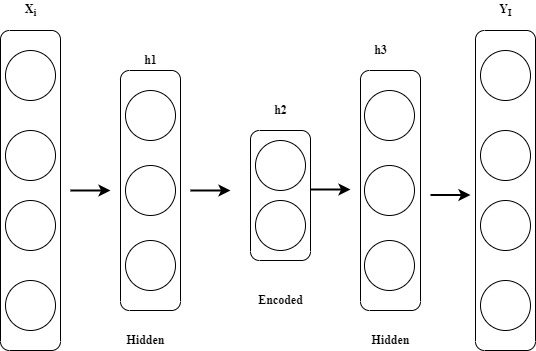
\includegraphics[width=4.2in,height=4.2in]{schematic_AE.jpg}
		\caption{DFD Diagram}
		\label{fig:EndorsersCommitters_Role}
	\end{Center}
\end{figure}
\end{Center}\par




\section*{4.5\hspace*{10pt}DataFlow Diagram for Deep Wavelet Autoencoder}
\addcontentsline{toc}{section}{4.5\hspace*{10pt}DataFlow Diagram for Deep Wavelet Autoencoder}
\begin{Center}
\begin{figure}[H]
	\begin{Center}
		\includegraphics[width=\linewidth]{deep.jpg}
		\caption{DFD Diagram}
		\label{fig:EndorsersCommitters_Role}
	\end{Center}
\end{figure}
\end{Center}\par

\section*{4.6\hspace*{10pt}Performance Analysis Result}
\addcontentsline{toc}{section}{4.6\hspace*{10pt}Performance Analysis Result Table}
\begin{Center}
\begin{figure}[H]
	\begin{Center}
		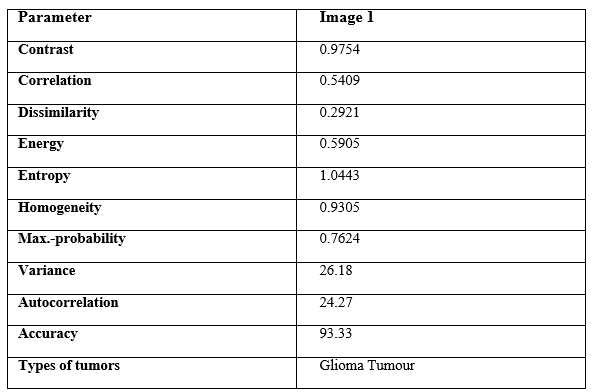
\includegraphics[width=\linewidth]{performance_analysis.png}
		\caption{Performance Analysis Result}
		\label{fig:EndorsersCommitters_Role}
	\end{Center}
\end{figure}
\end{Center}\par

\section*{4.7\hspace*{10pt}Model Analysis Result}
\addcontentsline{toc}{section}{4.7\hspace*{10pt}Model Analysis Result Table}
\begin{Center}
\begin{figure}[H]
	\begin{Center}
		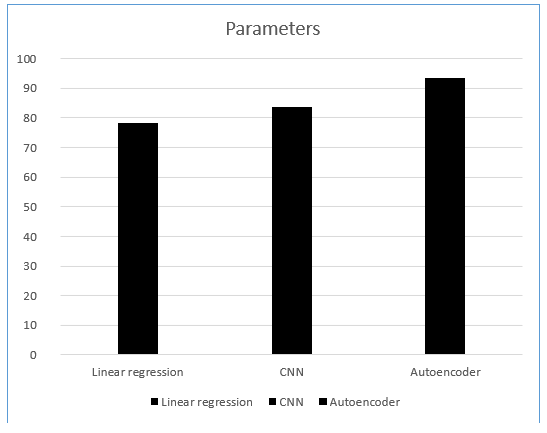
\includegraphics[width=\linewidth]{graph.png}
		\caption{Model Analysis Result}
		\label{fig:EndorsersCommitters_Role}
	\end{Center}
\end{figure}
\end{Center}\par


















 %%%%%%%%%%%%  Starting New Page here %%%%%%%%%%%%%%

\newpage

\vspace{\baselineskip}
\vspace{\baselineskip}

\vspace{\baselineskip}

\vspace{\baselineskip}

\vspace{\baselineskip}

\vspace{\baselineskip}

\vspace{\baselineskip}

\vspace{\baselineskip}

\vspace{\baselineskip}
\chapter{OTHER SPECIFICATIONS}\par



 %%%%%%%%%%%%  Starting New Page here %%%%%%%%%%%%%%

\newpage

\vspace{\baselineskip}\section*{5.1\hspace*{10pt}Advantages}
\addcontentsline{toc}{section}{5.1\hspace*{10pt}Advantages}
\( \hspace{0.5cm}\)
\begin{enumerate}
	\item As technology is being considered as a major part in field of medical sciences as well, this model shall help with the preliminary analysis.

    \item Being one of its kind in the entire country, the recommendation system we propose will be bringing in patients to the Hospitals  as per the severity and would reduce the time of examination.\par

	\item Based on this model. One can even track the history of a particular patient and make reports accordingly.\par
	\par
    
\end{enumerate}\par

\section*{5.2\hspace*{10pt}Limitations}
\addcontentsline{toc}{section}{5.2\hspace*{10pt}Limitations}
\begin{enumerate}
	\item \textbf {Written Evaluation }The model has not been taught to evaluate written reviews such as any written changes/suggestions, or other types of remarks. Because the processes necessary for evaluation differ from one patient to the next, they cannot be adequately assessed. The lack of a dataset has become a significant restriction.\par

	\item \textbf {Decentralization} Multiple hospitals as nodes are needed to make the health profile truly de-central.
	\par

\end{enumerate}\par


\vspace{\baselineskip}


 %%%%%%%%%%%%  Starting New Page here %%%%%%%%%%%%%%

\newpage

\vspace{\baselineskip}
\vspace{\baselineskip}

\vspace{\baselineskip}

\vspace{\baselineskip}

\vspace{\baselineskip}

\vspace{\baselineskip}

\vspace{\baselineskip}

\vspace{\baselineskip}

\vspace{\baselineskip}
\chapter{CONCLUSION AND FUTURE WORK}\par


\vspace{\baselineskip}

\vspace{\baselineskip}

\vspace{\baselineskip}

\vspace{\baselineskip}

\vspace{\baselineskip}

\vspace{\baselineskip}

\vspace{\baselineskip}

\vspace{\baselineskip}

\vspace{\baselineskip}

\vspace{\baselineskip}
\vspace{\baselineskip}\section*{6.1\hspace*{10pt}Conclusion }
\addcontentsline{toc}{section}{6.1\hspace*{10pt}Conclusion }
There is no proper tumor detection system as of now in the sector of medical
sciences, with the help of technology human errors would be minimised and the
whole system will be data driven with zero data manipulation and self feeding
data after some period of time.
\par With the help of this, we can do preliminary analysis and this model would be able
to give medical analysed results to the patients depending on his or her severity
of tumour.


\vspace{\baselineskip}\section*{6.2\hspace*{10pt}Future Work }
\addcontentsline{toc}{section}{6.2\hspace*{10pt}Future Work }
\par With this model, ML + web, we would look forward for tumour diagnosis not just
from MRI but also from blood cells and CT scan images as well.
With possible inclusion of these two, not just tumour any other anomalies in the
brain can be classified as well helping with initial diagnosis.
\vspace{\baselineskip}

\vspace{\baselineskip}

\vspace{\baselineskip}

\vspace{\baselineskip}

\vspace{\baselineskip}

\vspace{\baselineskip}

\vspace{\baselineskip}

\vspace{\baselineskip}

\vspace{\baselineskip}

\vspace{\baselineskip}

\vspace{\baselineskip}

\vspace{\baselineskip}

\vspace{\baselineskip}

\vspace{\baselineskip}

\vspace{\baselineskip}

\vspace{\baselineskip}

\vspace{\baselineskip}

\vspace{\baselineskip}

\vspace{\baselineskip}

\vspace{\baselineskip}

\vspace{\baselineskip}

\vspace{\baselineskip}

\vspace{\baselineskip}

\vspace{\baselineskip}


\vspace{\baselineskip}
\begin{appendices}
\setlength{\parskip}{15.0pt}
\chapter{FEASIBILITY ANALYSIS}\par

\setlength{\parskip}{9.96pt}
\section*{7.1\hspace*{10pt}Feasibility}
\addcontentsline{toc}{section}{1\hspace*{10pt}Feasibility}
\begin{enumerate}
    \item Dataset :
    The MRI scanned and verfied images from a kaggle.com project  was used for the recommendation system. The  attributes from the images  are required from the patients to make up the data. Each attributes receives a numerically determined score as well as one or more human ratings.
    \item Data Extraction:
    Patients' reviews might be taken on in a digital format. This response should be in string format so that it may be used as input for our model. Further data-cleaning and extraction takes place for extracting useful insights.
  
\end{enumerate}
\newpage
\section*{7.2\hspace*{10pt}Output and Results}
\addcontentsline{toc}{section}{2\hspace*{10p}Output and Results}

\section*{7.2.1\hspace*{10pt}Initial Page}
\addcontentsline{toc}{section}{2.1\hspace*{10pt}Initial Page}
\begin{Center}
\begin{figure}[H]
	\begin{Center}
		
\includegraphics[width=\linewidth]{initial_page.jpeg}
		\caption{1st page to select MRI }
		\label{fig:EndorsersCommitters_Role}
	\end{Center}
\end{figure}
\end{Center}\par

\section*{7.2.2\hspace*{10pt}Tumor found}
\addcontentsline{toc}{section}{2.1\hspace*{10pt}Tumor Found Result}
\begin{Center}
\begin{figure}[H]
	\begin{Center}
		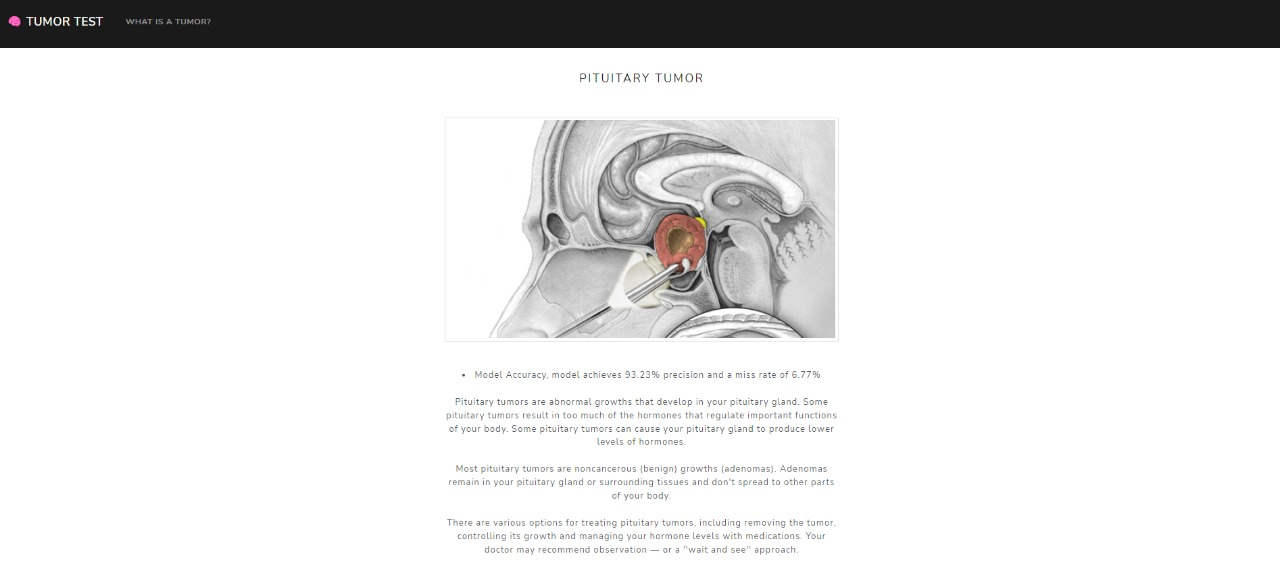
\includegraphics[width=\linewidth]{tumor_found_type_.jpeg}
		\caption{Detected Tumor and the type }
		\label{fig:EndorsersCommitters_Role}
	\end{Center}
\end{figure}
\end{Center}\par

\section*{7.2.3\hspace*{10pt}No Tumor}
\addcontentsline{toc}{section}{2.1\hspace*{10pt}No tumor Result}
\begin{Center}
\begin{figure}[H]
	\begin{Center}
		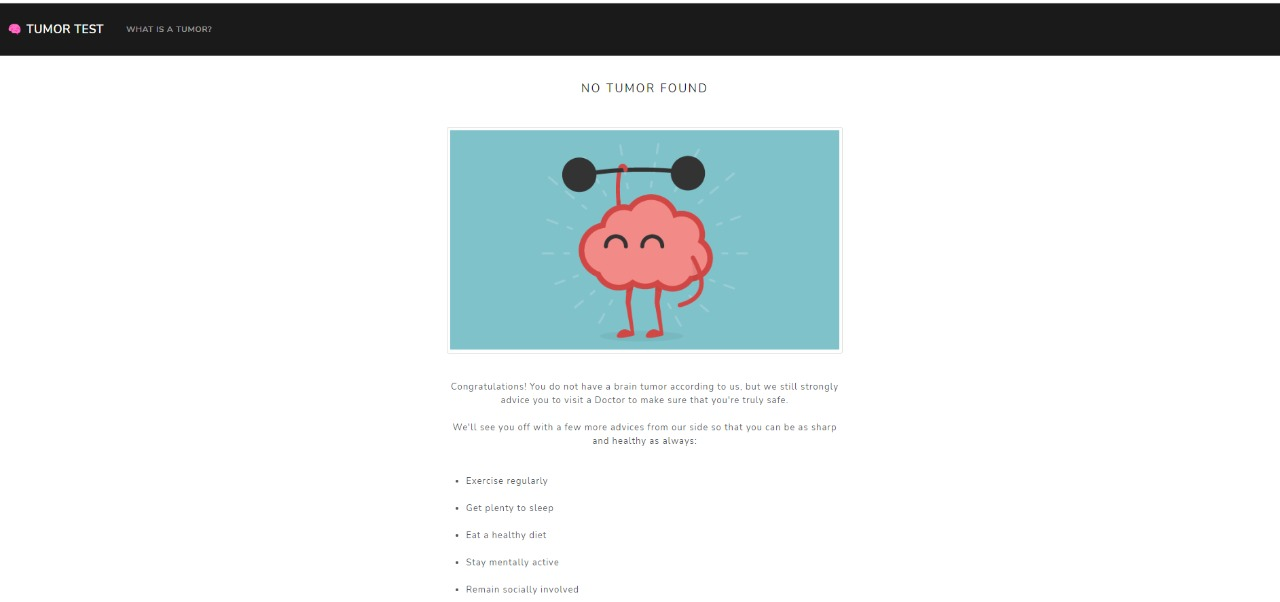
\includegraphics[width=\linewidth]{no_detected.jpeg}
		\caption{1st page to select MRI }
		\label{fig:EndorsersCommitters_Role}
	\end{Center}
\end{figure}
\end{Center}\par

\vspace{\baselineskip}

\vspace{\baselineskip}

\vspace{\baselineskip}

\vspace{\baselineskip}

\vspace{\baselineskip}

\vspace{\baselineskip}

\setlength{\parskip}{15.0pt}
\setlength{\parskip}{9.96pt}
\setlength{\parskip}{15.0pt}
\chapter{PLAGIARISM REPORT}\par

\vspace{\baselineskip}
\setlength{\parskip}{9.96pt}


%%%%%%%%%%%%%%%%%%%% Figure/Image No: 12 starts here %%%%%%%%%%%%%%%%%%%%



%%%%%%%%%%%%%%%%%%%% Figure/Image No: 12 Ends here %%%%%%%%%%%%%%%%%%%%

\par


\vspace{\baselineskip}

\vspace{\baselineskip}

\vspace{\baselineskip}

\vspace{\baselineskip}

\vspace{\baselineskip}

\vspace{\baselineskip}

\vspace{\baselineskip}

\vspace{\baselineskip}

\vspace{\baselineskip}

\vspace{\baselineskip}

\end{appendices}

\vspace{\baselineskip}

\vspace{\baselineskip}

\vspace{\baselineskip}

\vspace{\baselineskip}

\vspace{\baselineskip}

\vspace{\baselineskip}
\setlength{\parskip}{15.0pt}
\chapter{REFERENCES}\par

\setlength{\parskip}{0.0pt}
\begin{enumerate}
    \item H. Kholidy and F. Baiardi, “CIDS: A framework for intrusion detection in
cloud systems,” in Ninth International Conference on InformationTechnology:
New Generations (ITNG), 2012, April 2012, pp. 379–385 \par
 \item C. C. Benson and V. L. Lajish, “Morphology based enhancement and skull
stripping of MRI brain images,” in Proceedings of the international Conference on Intelligent Computing Applications (ICICA ’14), pp. 254–257, Tamilnadu, India, March 201\par

 \item S. Z. Oo and A. S. Khaing, “Brain tumor detection and segmentation using
watershed segmentation and morphological operation,” International Journal
of Research in Engineering and Technology, vol. 3, no. 3, pp. 367–374, 2014.\par

 \item G. Anandgaonkar, G. Sable, 2014. Brain tumor detection and identification post contrast MR images using cluster-based segmentation. International
Journal of Science and Research, 3(4), 814-7 \par
    
    \item Nilesh Bhaskarrao Bahadure, Arun Kumar Ray, Har Pal Thethi, “Image
Analysis for MRI Based Brain Tumor Detection and Feature Extraction Using
Biologically Inspired BWT and SVM”, International Journal of Biomedical
Imaging Volume 2017\par

	\item Be ̧sik, Saliha  ̇Irem, ” DESIGN AND DEVELOPMENT OF MEDICAL REC-OMMENDATION SYSTEM FOR HOME CARE SER-VICE FOR GERIATRICS”.\par

	\item Kevin Clauson and Peng Zhang, ”The  HealthChain  Blockchain  for  Electronic  HealthRecords: Development Study”, Lecture Notes in Computer Science\par

	\item https://www.mdpi.com/2076-3417/7/10/966/pdf
\par

	\item  https://journals.sagepub.com/doi/full/10.1177/1460458219866350
\par
        
    \item https://etd.lib.metu.edu.tr/upload/12619648/index.pdf
\par
    
    \item https://www.ncbi.nlm.nih.gov/pmc/articles/PMC7864769/
\par
 \item 	R. Roslan, N. Jamil, and R. Mahmud, “Skull stripping magnetic resonance images brain images: region growing versus mathematical morphology,” International Journal of Computer Information Systems and Industrial Management Applications, vol. 3, pp. 150– 158, 2011.
\par
 \item  Z. Oo and A. S. Khaing, “Brain tumor detection and segmentation using
watershed segmentation and morphological operation,” International Journal
of Research in Engineering and Technology, vol. 3, no. 3, pp. 367–374, 2014
\par
 \item A. Demirhan, M. Toru, and I. Guler, “Segmentation of tumor  and edema along with healthy tissues of brain using wavelets and neural networks,” IEEE Journal of Biomedical and Health Informatics, vol. 19, no. 4, pp. 1451–1458, 2015.
\par
 \item 	J. C. Buckner, P. D. Brown, B. P. O’Neill, F. B. Meyer , C. J. Wetmore,J. H Uhm, "Central nervous system tumors." In Mayo Clinic Proceedings,Vol. 82, No. 10, pp. 1271- 1286, October 2007.
\par
 \item https://etd.lib.metu.edu.tr/upload/12619648/index.pdf
\par
 \item 	DICOM Samples Image Sets, http://www.osirix-viewer.com/.
\par
 \item N. Gordillo, E. Montseny, and P. Sobrevilla, “State of the art survey on MRI brain tumor segmentation,”Magnetic Resonance Imaging, vol. 31, no. 8, pp. 1426–1438, 2013.
\par
 \item 	Nandi, A. (2016, April 11) Retrieved from http://ieeexplore.ieee.org/document/7449892/
\par
\end{enumerate}\par


\vspace{\baselineskip}
\setlength{\parskip}{9.96pt}

\printbibliography
\end{document}